\resizebox{\linewidth}{!}{%
\begin{tikzpicture}[
  imgnode/.style={inner sep=0pt, draw=black!35, line width=1.0pt},
  boxnode/.style={draw=black!70, rounded corners=2pt, minimum height=1.0cm, minimum width=1.5cm, align=center, font=\small, fill=black!3, inner sep=4pt},
  arr/.style={-{Latex[length=2.2mm,width=1.6mm]}, very thick, black!65},
  titletext/.style={font=\Large\bfseries},
  captiontext/.style={font=\small\itshape, align=center, text width=10cm},
  annot/.style={font=\small\itshape, align=center},
]

% ---------- left: passive perception ----------
% same crop as the active side's "what it sees" -- the passive model is simply
% handed, for free, the exact view the active agent had to act to obtain.
% Width matches scene3p below so both top rows share the same height, which
% keeps the two titles/dividers aligned without needing cross-group coordinate
% lookups.
\node[imgnode] (fullscene) {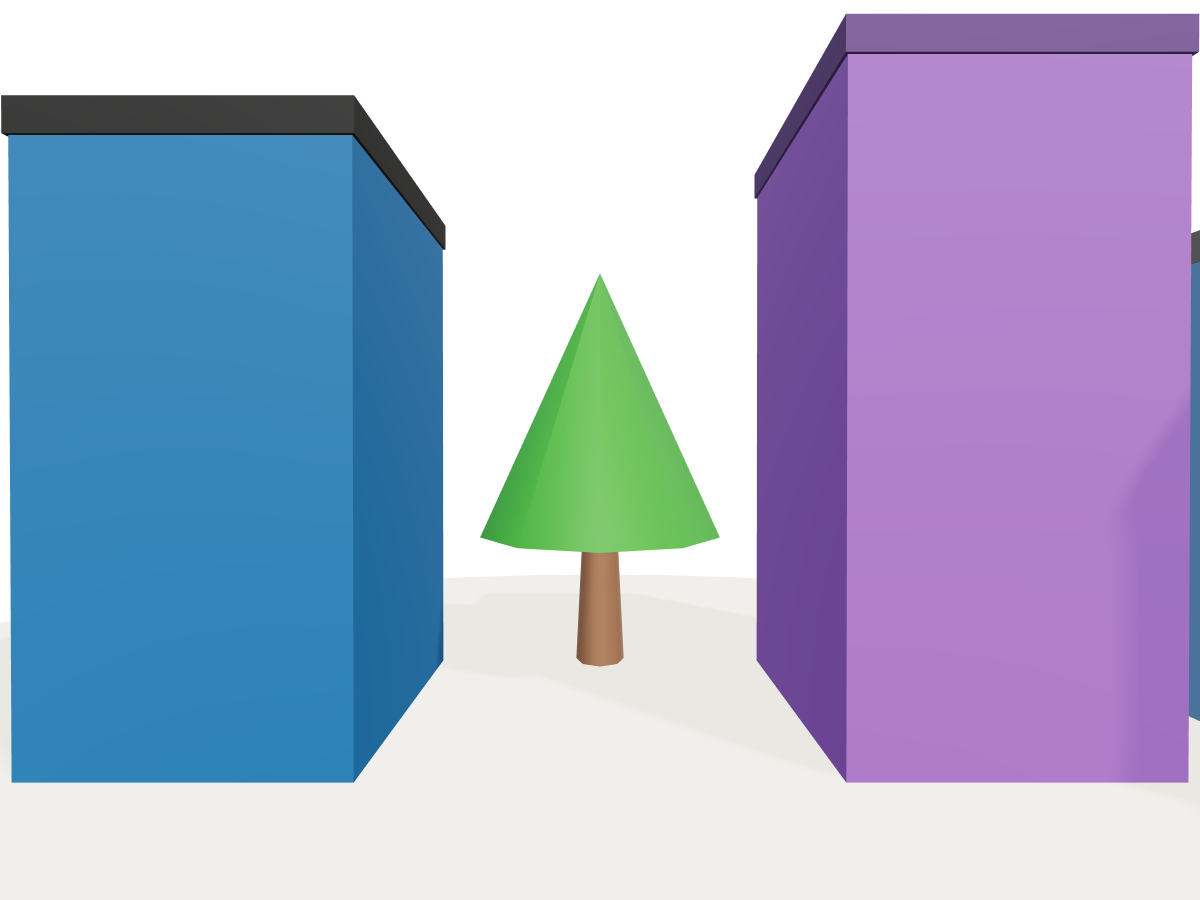
\includegraphics[width=3.1cm]{img/main/three/renders/robot_scene_1p.png}};
\node[boxnode, right=1cm of fullscene] (model1) {Model};
\node[right=1cm of model1, font=\bfseries] (out1) {\textquotedblleft tree\textquotedblright};

\draw[arr] (fullscene) -- (model1);
\draw[arr] (model1) -- (out1);

\node[fit=(fullscene)(model1)(out1), inner sep=0pt] (leftgroup) {};
\node[titletext, above=1.0cm of leftgroup] (lefttitle) {Passive perception};
\node[captiontext, below=0.15cm of lefttitle] (leftcap) {complete visual information provided};
\node[captiontext, below=0.45cm of leftgroup] (leftcap2) {(single feed-forward pass)};

% ---------- right: active embodied vision ----------
% anchored off "out1" (the true rightmost element of the left group), not
% "fullscene" -- anchoring off fullscene alone let this group overlap model1/out1.
\node[imgnode, right=1.5cm of out1] (scene3p) {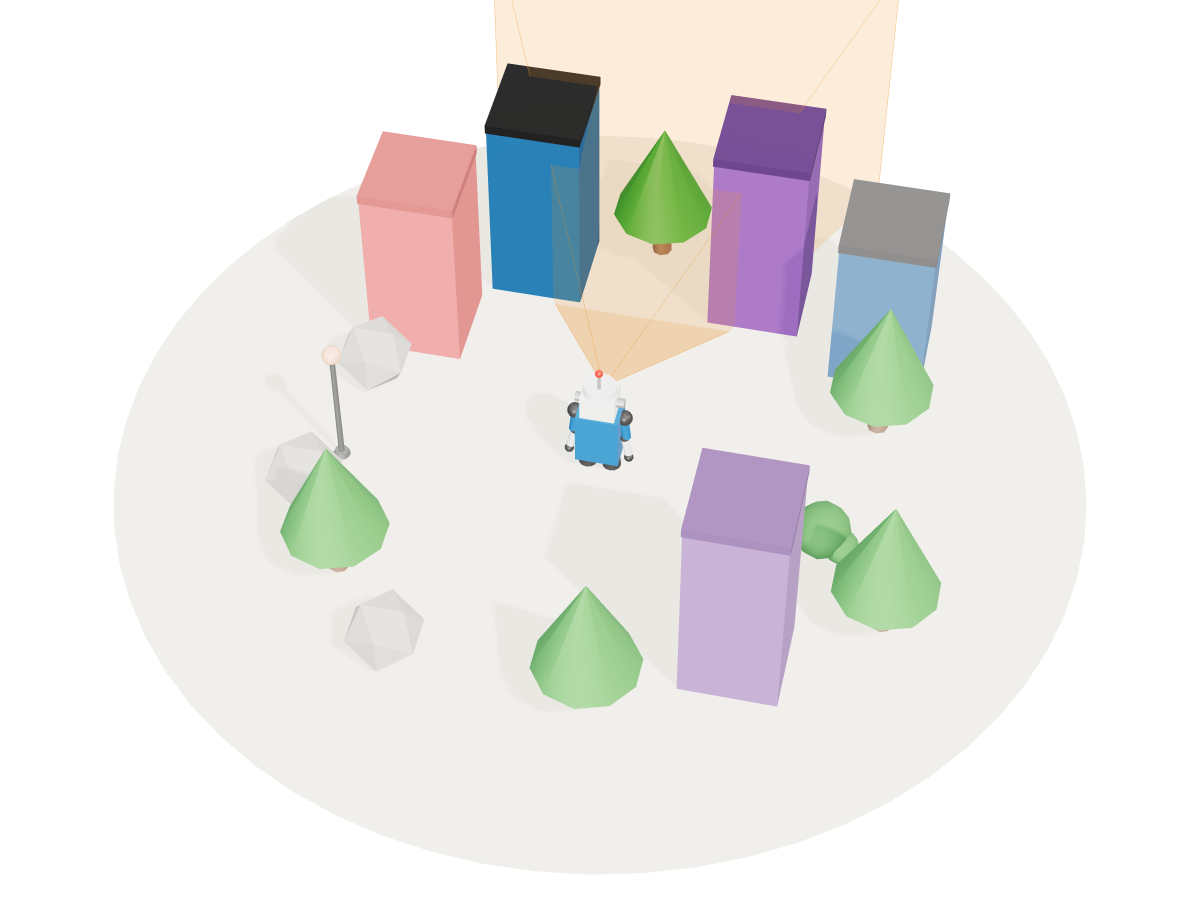
\includegraphics[width=4cm]{img/main/three/renders/robot_scene_3p.png}};
\node[imgnode, right=1cm of scene3p, label=above:camera view] (scene1p) {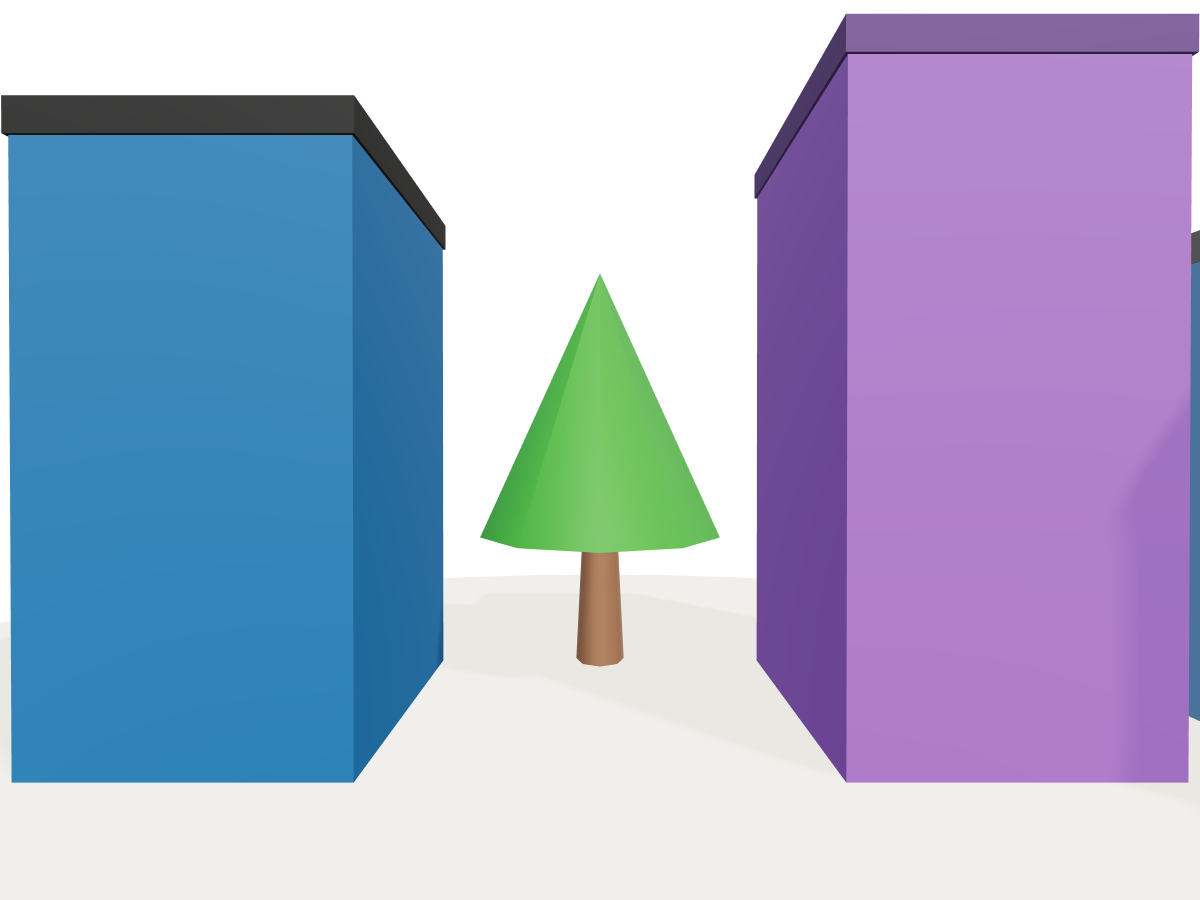
\includegraphics[width=2cm]{img/main/three/renders/robot_scene_1p.png}};
\node[boxnode, right=1cm of scene1p] (model2) {Model};

\draw[arr] (scene3p) -- (scene1p);
\draw[arr] (scene1p) -- (model2);

% the action closes the loop: model -> scene (it moves/looks, producing the
% next observation). The action text sits just below this arrow, as its caption.
% loopbottom is anchored below scene3p (not model2) so the final vertical run
% into scene3p.south is always comfortably longer than the corner-rounding
% radius -- too short a run there left the arrowhead angled instead of pointing
% straight up into the image.
\coordinate (loopbottom) at ($(scene3p.south)+(0,-0.5)$);
\coordinate (loopcorner) at (model2.south |- loopbottom); % x of model2.south, y of loopbottom
\draw[arr, rounded corners=7pt] (model2.south) -- (loopcorner) -- (loopbottom) -- (scene3p.south);

\path (scene3p.south) -- (model2.south) coordinate[midway] (loopmid);
\node[align=center, font=\bfseries\footnotesize, anchor=north] (actA) at ($(loopmid)+(-0,-1.0)$) {move forward and look to the right};

% \draw[decorate, decoration={brace, amplitude=3pt, mirror}, thin, black!55]
%   (actA.south west) -- (actA.south east) node[midway, below=4pt, annot] {global};
% \draw[decorate, decoration={brace, amplitude=3pt, mirror}, thin, black!55]
%   (actB.south west) -- (actB.south east) node[midway, below=4pt, annot] {local};

\node[fit=(scene3p)(scene1p)(model2)(actA), inner sep=0pt] (rightgroup) {};
\node[titletext, above=1cm of rightgroup] (righttitle) {Active embodied vision};
\node[captiontext, text width=10.0cm, below=0.15cm of righttitle] (rightcap) {the agent acts to decide what to observe next};
\node[captiontext, below=0.45cm of rightgroup] (rightcap2) {(perceive $\to$ act $\to$ repeat)};

% ---------- divider ----------
% a genuinely thin rule (table-style), spanning from above the titles to below
% both captions -- generous height since it must clear the (lower) right side.
\node[fill=black!45, inner sep=0pt, minimum width=0.4pt, minimum height=7.0cm, anchor=north,
      right=0.85cm of leftgroup.east, yshift=-.5cm] {};

\end{tikzpicture}%
}
